% Estado del arte
\chapter{Estado del arte} \label{ch:estado}
\section{Tecnologías de virtualización} \label{sec:virt}
Se podría decir que la virtualización es ya uno de los pilares fundamentales del mundo IT debido a las grandes ventajas que proporciona. Previo al desarrollo de las tecnologías y tipos de virtualización disponibles, es conveniente explicar en qué consiste la virtualización, que no es más que una representación mediante software de un entorno físico o recurso tecnológico, como pueden ser aplicaciones, servidores o almacenamiento.~\cite{virt1} 

Gracias a esta tecnología, es posible contar con varios ordenadores virtuales en el mismo hardware, donde cada uno de ellos puede interactuar de forma independiente y ejecutar sistemas operativos o aplicaciones diferentes mientras comparten los recursos de una sola máquina host. Al crear varios recursos a partir de un único equipo o servidor, la virtualización mejora la escalabilidad y las cargas de trabajo, al tiempo que permite usar menos servidores y reducir el consumo de energía, los costos de infraestructura y el mantenimiento.

En función del sistema a simular, podemos encontrar diferentes categorías~\cite{virt2}, un ejemplo es la virtualización de red, que consiste en crear redes virtuales sobre redes físicas o reproducir completamente redes físicas en software. Otro ejemplo sería la virtualización de almacenamiento, que combina varios dispositivos de almacenamiento en red, con la apariencia de una única unidad o dispositivo de almacenamiento, accesible por varios usuarios. Podríamos enumerar más tipos de virtualización, pero en lo que a este trabajo respecta vamos a centrarnos en la virtualización de software, que separa las aplicaciones del hardware y el sistema operativo, y en la que distinguimos dos subtipos: virtualización mediante hipervisor y virtualización en contenedores.

\subsection{Virtualización mediante hipervisor} \label{sec:hiperv}
Una máquina virtual es un software que ejecuta programas o procesos como si fuera la máquina física. Es decir, se abstrae el hardware y se representa con una capa de software que proporciona una interfaz igual que el hardware, de forma que sobre ella podemos instalar uno o varios sistema operativos invitados o \textit{guests} distintos. Esta capa de software también se encarga de repartir y aislar los recursos del host entre las VM\footnote{Virtual Machine}, de manera que el host queda protegido si falla una VM, y las VM estén protegidas entre ellas. Pues bien, cuando hablamos de esta capa de software estamos hablando de lo que se conoce como hipervisor. 

Como ya se ha mencionado, un hipervisor es una capa intermedia de software que permite al ordenador anfitrión prestar soporte a varias máquinas virtuales mediante el uso compartido de sus recursos. Cuando se ejecuta una instrucción en el SO\footnote{Sistema Operativo} invitado, el hipervisor la coje y la ejecuta en el SO anfitrión. En este proceso, el SO no diferencia entre ejecutar procesos en la máquina virtual o en la física, lo que representa plenamente el concepto de virtualización.

Dentro de los hipervisores~\cite{virt3}, podemos distinguir dos tipos. El primero es el Tipo 1, conocido también como hipervisor nativo o \textit{bare-metal}. Este hipervisor se ejecuta directamente sobre el hardware en lugar de un SO clásico. Todos los hipervisores necesitan algunos elementos del sistema operativo (por ejemplo, el administrador de memoria, el programador de procesos, la pila de entrada o salida [E/S], los controladores de dispositivos, entre otros) para ejecutar las máquinas virtuales. Por tanto, este hipervisor es equivalente a un SO con un poco de información adicional que le permite gestionar los SO invitados. Es muy común encontrarlos en centros de datos, por la eficiencia que supone el ahorrar una capa de software.

Los hipervisores de Tipo 2 se ejecutan sobre el SO anfitrión como una capa de software o aplicación. Están orientados a usuarios individuales que buscan ejecutar varios SO en el mismo ordenador. La ejecución de una VM sobre un hipervisor de este tipo es más lenta que en un hipervisor de Tipo 1.

\begin{figure}[h]
\centering
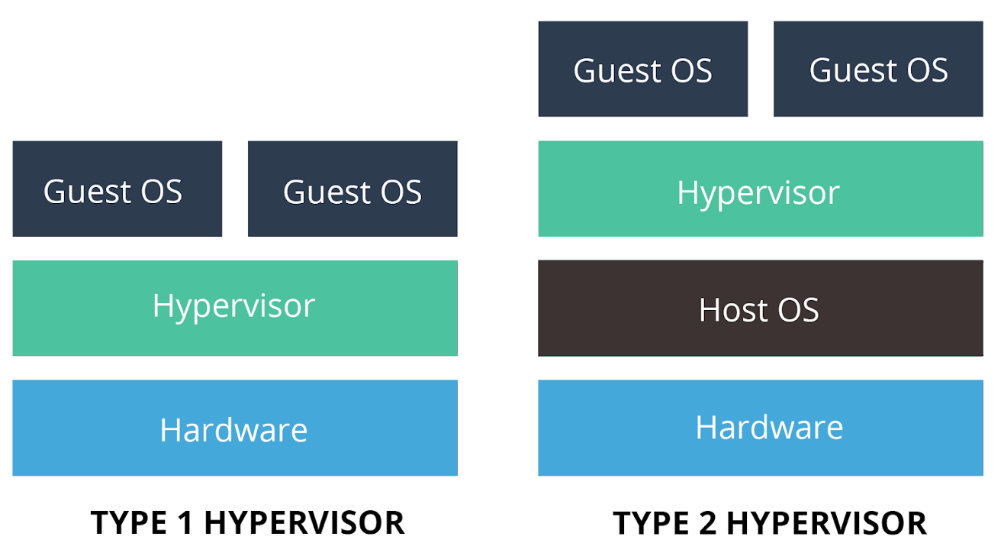
\includegraphics[width=0.7\textwidth]{../imgs/EdA/hipervisor.jpg}
\caption{Tipos de hipervisor}
\label{fig:hipervtypes}
\end{figure}

A continuación se presentan algunas tecnologías que emplean este tipo de virtualización.
\clearpage

\subsubsection{KVM}
KVM (Kernel Virtual Machine)~\cite{kvm} es una tecnología de virtualización open source que convierte el kernel de Linux en un hipervisor de Tipo 1 que se puede usar para la virtualización. Las KVM tienen todos los elementos necesarios de un SO porque forman parte del kernel de Linux. Cada máquina virtual se implementa como un proceso habitual de Linux. Al ser un hipervisor de Tipo 1 ofrece un mejor rendimiento. 

\begin{figure}[h]
\centering
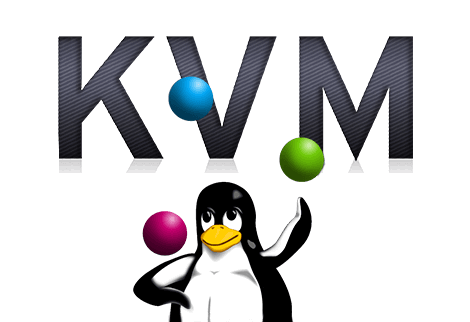
\includegraphics[width=0.3\textwidth]{../imgs/EdA/kvm.png}
\caption{Logo de KVM}
\label{fig:kvm}
\end{figure}

La configuración de la máquina virtual creada se almacena internamente en un fichero XML, el cual es posible editar manualmente a posteriori si se quiere hacer algún cambio. KVM nos permite disfrutar de las ventajas del software open source: no habrá restricciones en cuanto a integración, como sí puede haberlas si se usa un software propietario como VMware; y es independiente de proveedores. Es posible instalar una GUI\footnote{Graphical User Interface} como virt-manager, que se apoya en la biblioteca libvirt (API de virtualización estándar de Linux), para facilitar su uso.

\subsubsection{VirtualBox}
VirtualBox~\cite{vbox} es desarrollado por Oracle, aunque es gratuito y open source al igual que KVM. Es un hipervisor de Tipo 2, por lo que ofrece un rendimiento inferior comparado con un Tipo 1. VirtualBox permite crear y cargar máquinas virtuales de una forma muy sencilla, lo que hace que sea la alternativa elegida por muchos usuarios. Su asistente ofrece algunos valores sugeridos para tipos específicos de máquinas virtuales durante la creación de estas, pero su gestión final se produce en una configuración posterior.

\begin{figure}[h]
\centering
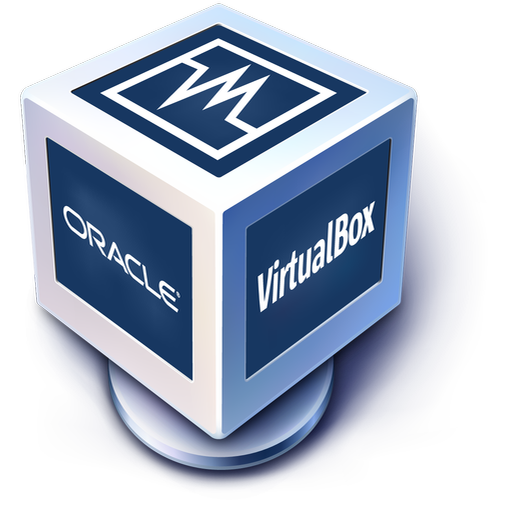
\includegraphics[width=0.2\textwidth]{../imgs/EdA/vbox.png}
\caption{Logo de VirtualBox}
\label{fig:vbox}
\end{figure}

Una ventaja de VirtualBox son las instantáneas, que permiten tomar una imagen de la máquina virtual en un momento dado. La imagen conserva la máquina virtual, lo que permite volver a ese momento específico.

VirtualBox ofrece un soporte muy completo. Tiene versiones para Windows, Linux, Macintosh y Solaris, y puede ejecutar un amplísimo número de sistemas operativos invitados, incluidos Windows, macOS, Linux, DOS, Solaris u OpenBSD.

\subsubsection{VMware}
VMware~\cite{vmware} es un software comercial, lo que significa que si queremos aprovechar al máximo todas sus herramientas y configuraciones, debemos pagar por la licencia de uso. Aquí vamos a hablar de VMware Workstation Player, que es el producto gratuito de VMware para virtualización de máquinas, orientado para uso personal, doméstico y sistema educativo. 

\begin{figure}[h]
\centering

\includegraphics[width=0.2\textwidth]{../imgs/EdA/vmware.png}
\caption{Logo de VMware}
\label{fig:vmware}
\end{figure}

En comparación con VirtualBox, VMware Workstation Player es una experiencia más fluida y ágil, y ofrece mejor soporte y estabilidad para una amplia gama de hardware. Está disponible para Windows y Linux y también admite todo tipo de sistemas invitados.~\cite{versus}

Además, VMware Workstation Player sí permite personalizar toda la configuración durante el proceso de creación de la máquina virtual. La diferencia no es mucha, pero significa que la máquina virtual está lista para ejecutarse después de finalizar el asistente, en lugar de tener que realizar más configuraciones una vez que se completa.

Por el contrario, no admite instantáneas o puntos de control. Puede suspender temporalmente el sistema operativo invitado para reanudar desde un punto específico, pero no es tan completo como la creación de un historial de imágenes para la máquina virtual.

\clearpage
\subsection{Virtualización en contenedores} \label{sec:cont}
La virtualización basada en contenedores, también llamada virtualización del sistema operativo, es una aproximación a la virtualización en la cual la capa de virtualización se ejecuta como una aplicación en el sistema operativo.

Un contenedor~\cite{cont1} es un conjunto de uno o más procesos aislados del resto del sistema, que acceden sólo a los recursos que se indican. El contenedor encapsula el programa específico y las librerías, mientras que utiliza el sistema operativo del host. Podemos distinguir entre dos tipos de contenedores:~\cite{cont2}

\begin{itemize}
	\item \textbf{A nivel de sistema operativo:} un sistema operativo completo se ejecuta en un espacio aislado dentro de la máquina host, compartiendo el mismo kernel.
	\item \textbf{A nivel de aplicación:} una aplicación o servicio, y los procesos mínimos requeridos por esa aplicación, se ejecutan en un espacio aislado dentro de la máquina host.
\end{itemize}

Al compartir el mismo kernel del sistema operativo host, un contenedor sólo puede ejecutar procesos en ese sistema operativo. Es decir, un contenedor que se ejecuta en un servidor de Linux, por ejemplo, solo puede ejecutar un sistema operativo Linux, mientras que tal y como habíamos comentado, un hipervisor emula el hardware, lo que permite que varios sistemas operativos (Windows o Linux) se ejecuten simultáneamente en un solo sistema. Además, esta compartición del núcleo hace que el nivel de aislamiento sea menor comparado con las máquinas virtuales, ya que al acceder todos los contenedores al mismo núcleo, si se explota una vulnerabilidad en el núcleo ésta afectaría a todo el sistema, incluidos todos los contenedores.

A cambio, con la virtualización basada en contenedores, no existe la sobrecarga asociada con tener a cada huésped ejecutando un sistema operativo completamente instalado. Este enfoque también puede mejorar el rendimiento porque hay un solo sistema operativo encargándose de los avisos de hardware.

Tal y como se ha mencionado previamente, los contenedores hacen uso del kernel del sistema operativo, del que cabe destacar las siguientes características necesarias para el correcto funcionamiento de este tipo de virtualización:~\cite{cont3}

\begin{itemize}
	\item \textbf{Grupos de control o cgroups.} Se encargan de gestionar los recursos del ordenador asignados a un proceso o conjunto de procesos, como pueden ser el número de \textit{slices} de tiempo de CPU asignadas a cada proceso, el límite de memoria a usar por proceso, los dispositivos de bloques de E/S… Es posible estructurar los recursos en jerarquía.
	\item \textbf{Namespaces.} Permiten aislar procesos entre sí. Los procesos de un contenedor se asignan a un namespace, y el sistema operativo aísla los recursos entre ese namespace y el resto. Hay diferentes tipos de namespace: de PID\footnote{Process Identifier}, que permiten mantener los mismos PIDs en diferentes contenedores; mount, para separar sistemas de ficheros; de red para aislar controladores de red… 
\end{itemize}

Los contenedores, por tanto, suponen una virtualización más ligera: usan menos recursos que las máquinas virtuales, además de proporcionar mayor flexibilidad y rapidez de arranque y despliegue. Esto último se debe a que, al usar el mismo kernel que el host, sólo están iniciando procesos, algo que es casi instantáneo y que hace muy fluida la ejecución de diferentes máquinas a la vez.

Para contextualizar con el apartado \ref{sec:hiperv}, se muestra una imagen comparativa de la estructura de un contenedor respecto a una máquina virtual:

\begin{figure}[h]
\centering
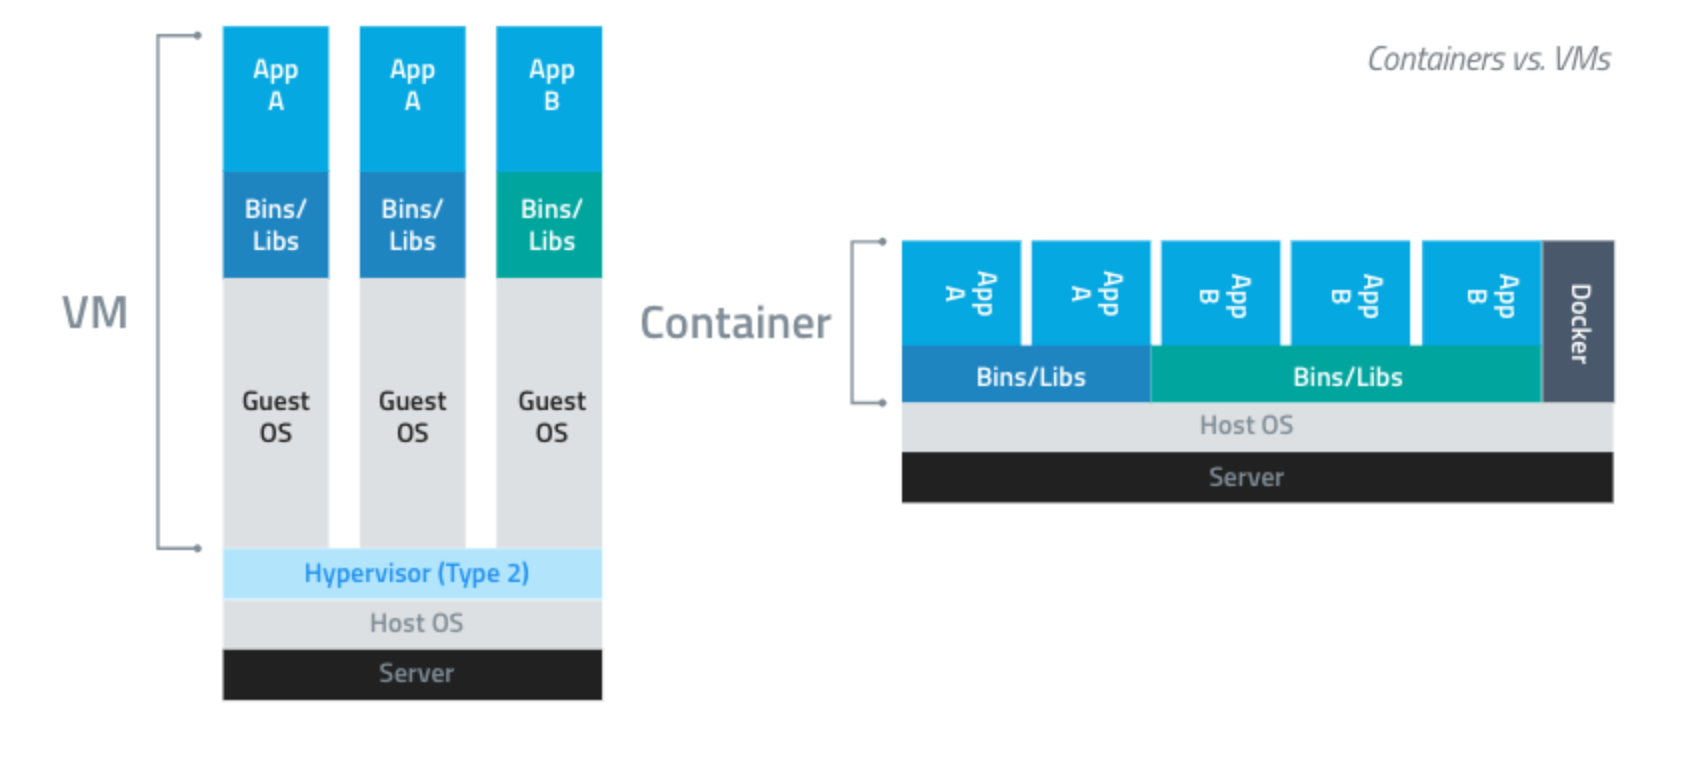
\includegraphics[width=\textwidth]{../imgs/EdA/VMvsCont.png}
\caption{Estructura de un contenedor vs VM}
\label{fig:VMvsDocker}
\end{figure}

\subsubsection{LXC}
LXC (Linux Containers)~\cite{lxc} es una plataforma de código abierto de contenedores a nivel de sistema operativo. Este tipo de contenedores hacen que un único host Linux actúe como varios host Linux. Esto es debido a que los contenedores LXC incluyen un sistema Linux prácticamente completo, similar a una VM, con su propio sistema de ficheros, espacio de red y aplicaciones. Su objetivo es recrear un entorno lo más parecido posible a una instalación de Linux, pero sin la necesidad de un kernel independiente. 

\begin{figure}[h]
\centering
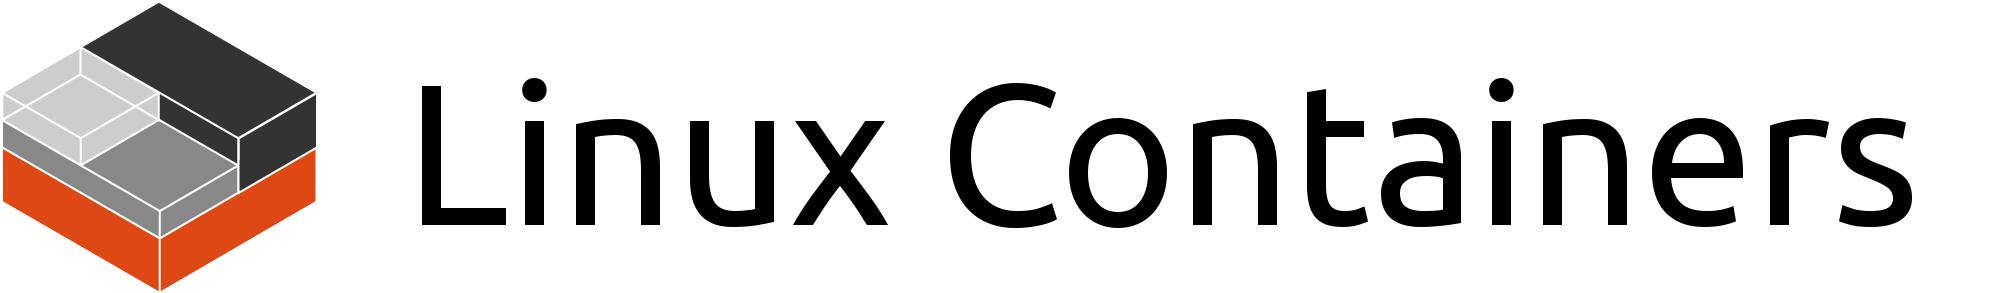
\includegraphics[width=0.5\textwidth]{../imgs/EdA/lxc.png}
\caption{Logo de LXC}
\label{fig:lxc}
\end{figure}

Chroot es un comando UNIX que permite ejecutar un proceso bajo un directorio raíz simulado, de manera que el proceso no puede acceder a archivos fuera de ese directorio. LXC es similar a un chroot, pero ofrece mucho más aislamiento. 

Para crear diferentes contenedores de sistema operativo, se emplean plantillas o templates. Las plantillas proporcionadas en LXC son scripts específicos de un sistema operativo.

LXC se suele usar junto a LXD. LXD ofrece una interfaz para gestionar contenedores LXC como si fueran máquinas virtuales, proporcionando snapshots y control de imágenes, además de otras funcionalidades que incrementan el potencial de LXC. Una de las ventajas principales de LXC es que es una tecnología sencilla de manejar.

\subsubsection{Docker}
Docker~\cite{docker1} es uno de los proyectos más conocidos y utilizados en este tipo de virtualización. Lejos de ser un sistema operativo como tal, esta plataforma de código abierto hace uso de las funciones de aislamiento de recursos del kernel de Linux para dar lugar a contenedores independientes. Está basada en Linux, pero en los últimos años se ha producido un desarrollo y actualmente también es posible su uso en Windows.

Los contenedores que proporciona Docker son a nivel de aplicación (puede ejecutar aplicaciones normales sin incluir un sistema operativo completo), y su implementación está basada en imágenes, lo que permite compartir una aplicación o un conjunto de servicios, con todas sus dependencias, en varios entornos.

Docker utiliza una arquitectura cliente-servidor. En este tipo de arquitectura, las tareas se reparten entre los proveedores de recursos o servicios, llamados servidores, y quienes demandan esos recursos o servicios, que son los clientes. Un sistema de contenedores Docker se compone principalmente de 5 elementos:~\cite{docker2}

\begin{itemize}
	\item \textbf{Demonio:} es el proceso principal de la plataforma.
	\item \textbf{Cliente:} binario que constituye la interfaz y que permite al usuario interactuar con el Demonio mediante CLI.
	\item \textbf{Imagen:} plantilla utilizada para crear el contenedor para la aplicación que queremos ejecutar.
	\item \textbf{Registros:} directorios donde se almacenan las imágenes, tanto de acceso público como privado. El más común es Docker Hub.
	\item \textbf{Contenedores:} carpetas donde se almacena todo lo necesario (librerías, dependencias, binarios, etc) para que la aplicación pueda ejecutarse de forma aislada.
\end{itemize}

Docker Engine es la aplicación cliente-servidor responsable de iniciar y parar los contenidos de una manera similar a como lo hace el hipervisor en una máquina virtual. A continuación se muestra una figura donde se muestran de forma gráfica las interacciones entre los ya mencionados componentes:
\begin{figure}[h]
\centering
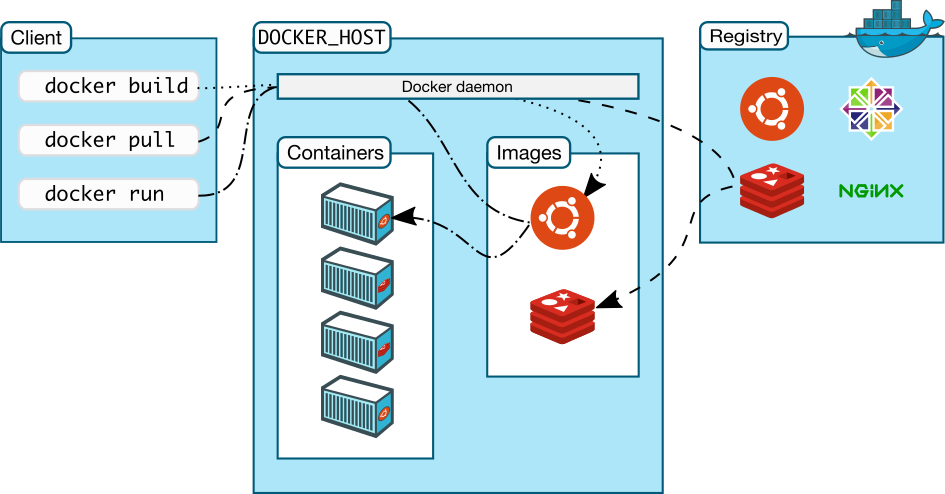
\includegraphics[width=0.8\textwidth]{../imgs/EdA/docker-arch.png}
\caption{Arquitectura del sistema de contenedores Docker}
\label{fig:docker-arch}
\end{figure}

En el ciclo de vida de un contenedor Docker podemos distinguir 5 estados principales:

\begin{itemize}
	\item \textbf{Created:} hace referencia a un contenedor que ha sido creado pero no arrancado.
	\item \textbf{Running/Started:} contenedor corriendo con todos sus procesos.
	\item \textbf{Paused:} contenedor cuyos procesos se han pausado usando la señal SIGSTOP de cgroups.
	\item \textbf{Stopped/Exited:} contenedor cuyos procesos se han parado. La diferencia con \textit{paused} es que se libera la memoria que estaban usando los procesos que han sido detenidos, usando la señal SIGKILL de cgroups. El sistema de ficheros se mantiene tal y como estaba en el momento que se detuvo el contenedor.
	\item \textbf{Deleted/Dead:} contenedor eliminado. Es posible recuperarlo durante un periodo de tiempo determinado.
\end{itemize}

\begin{figure}[h]
\centering
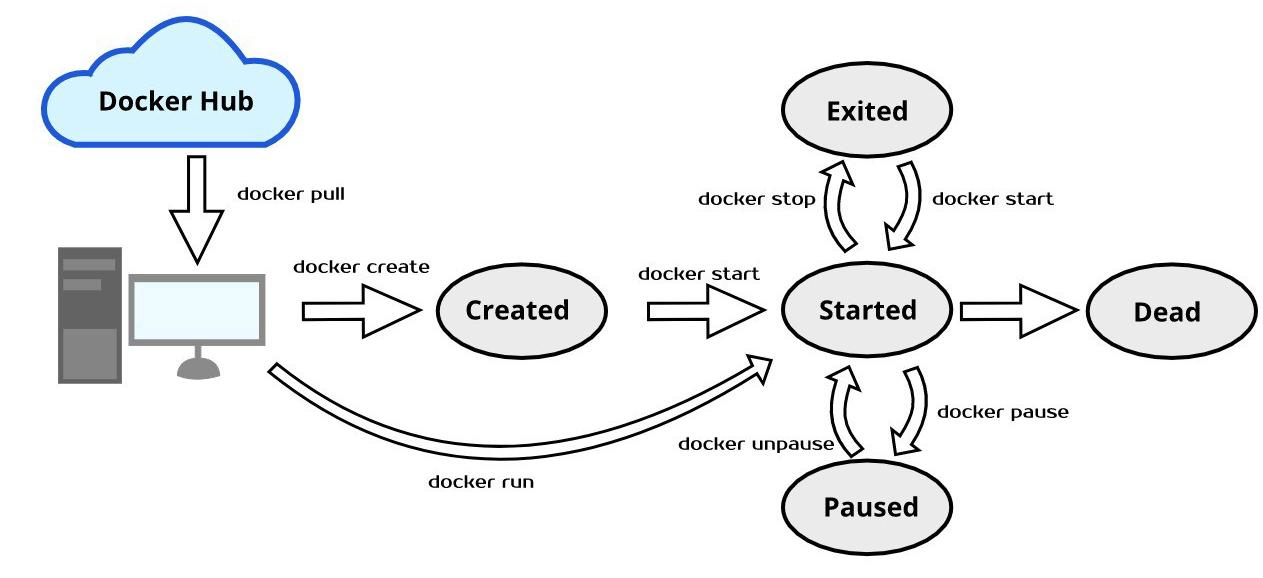
\includegraphics[width=0.8\textwidth]{../imgs/EdA/docker-life.jpeg}
\caption{Ciclo de vida de los contenedores Docker}
\label{fig:docker-life}
\end{figure}

Como se puede apreciar en la figura, Docker permite gestionar el estado de los contenedores de forma sencilla mediante la CLI\footnote{Command Line Interface}, algunas de sus órdenes más destacadas son:

\begin{lstlisting}[language=bash]
  $ docker pull #permite descargar una imagen de un repositorio
  $ docker create #crea un nuevo contenedor, pero no lo arranca 
  $ docker start #arranca contenedores parados
  $ docker run #es equivalente a create + start
  $ docker stop #detiene los procesos corriendo en un contenedor  
  $ docker pause #pausa los procesos corriendo en un contenedor
  $ docker unpause #reanuda la ejecucion de los procesos pausados
  $ docker rm #elimina los procesos y el contenedor donde corrian
\end{lstlisting}

\begin{figure}[h]
\centering

\includegraphics[width=0.2\textwidth]{../imgs/EdA/docker.png}
\caption{Logo de Docker}
\label{fig:docker-logo}
\end{figure}

\subsubsection{Diferencias entre LXC y Docker}
Con todo esto, podemos sacar varias conclusiones importantes acerca de estos dos tipos de contenerización, que condicionarán la elección de uno u otro en función de su uso. La principal sería que mientras que con LXC se virtualiza un sistema operativo completo, con Docker se virtualizan aplicaciones. Además, los contenedores LXC sólo permiten virtualizar entornos Linux y no se pueden portar entre máquinas, mientras que Docker permite portar entre máquinas e incluso plataformas. Esto último es algo relevante puesto que si en algún momento fuese necesario migrar a otro entorno, gracias a la portabilidad de Docker nos ahorraremos el tener que instalar en este nuevo entorno todas aquellas aplicaciones que normalmente usemos. 

Finalmente, también cabe recalcar que LXC proporciona un menor aislamiento del sistema operativo respecto a Docker. Al virtualizar sistemas operativos completos y aislados dentro del mismo host, debe haber usuario root y llamadas al propio sistema operativo (si no fuese así, estaríamos ante un sistema «recortado» porque no se podrían hacer determinadas cosas). Docker sirve para virtualizar aplicaciones dentro de un mismo host, por lo que el nivel de acceso root sí puede estar más limitado y controlado, lo que lo hace más seguro.

\vspace{0.2cm}
\begin{figure}[h]
\centering
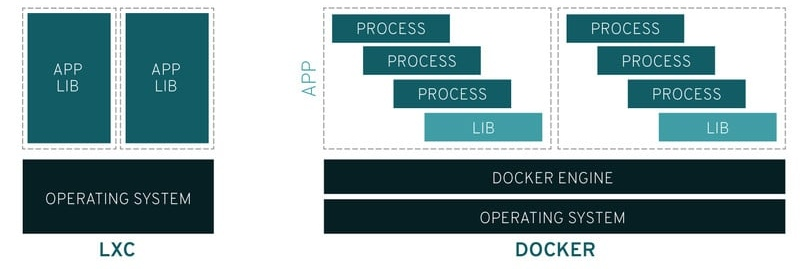
\includegraphics[width=0.8\textwidth]{../imgs/EdA/LXCvsDocker.jpg}
\caption{Estructura de Docker vs LXC}
\label{fig:docker-life}
\end{figure}
\clearpage

\section{Tecnologías de aprovisionamiento} \label{ch:aprov}
\subsection{Aprovisionamiento estático} \label{sec:est}
\subsubsection{Docker}
\subsubsection{Vagrant}
\subsection{Aprovisionamiento dinámico} \label{sec:din}
\subsubsection{Chef}
\subsubsection{Ansible}
\section{Tecnologías de orquestación} \label{ch:orq}
\subsubsection{Docker Compose}
\subsubsection{Kubernetes}
\subsubsection{Terraform}
\subsubsection{Tecnologías de orquestación de proveedores cloud}
